\documentclass[9pt,twocolumn,twoside]{pnas-new}
% Use the lineno option to display guide line numbers if required.
% Note that the use of elements such as single-column equations
% may affect the guide line number alignment. 


\templatetype{pnasresearcharticle} % Choose template 
% {pnasresearcharticle} = Template for a two-column research article
% {pnasmathematics} = Template for a one-column mathematics article
% {pnasinvited} = Template for a PNAS invited submission

\usepackage[algo2e]{algorithm2e}

\usepackage{subfig}
\title{On cloning machine intelligence}
% Use letters for affiliations, numbers to show equal authorship (if applicable) and to indicate the corresponding author
\author[a,c,1]{Najeeb Khan}
\author[b,1,2]{Mridul Gupta} 
\author[a]{Debarka Sengupta}

\affil[a]{Affiliation One}
\affil[b]{Affiliation Two}
\affil[c]{Affiliation Three}

% Please give the surname of the lead author for the running footer
\leadauthor{Lead author last name} 

% Please add here a significance statement to explain the relevance of your work
\significancestatement{Authors must submit a 120-word maximum statement about the significance of their research paper written at a level understandable to an undergraduate educated scientist outside their field of specialty. The primary goal of the Significance Statement is to explain the relevance of the work in broad context to a broad readership. The Significance Statement appears in the paper itself and is required for all research papers.}

% Please include corresponding author, author contribution and author declaration information
\authorcontributions{Please provide details of author contributions here.}
\authordeclaration{Please declare any conflict of interest here.}
\equalauthors{\textsuperscript{1}A.O.(Author One) and A.T. (Author Two) contributed equally to this work (remove if not applicable).}
\correspondingauthor{\textsuperscript{2}To whom correspondence should be addressed. E-mail: author.two\@email.com}

% Keywords are not mandatory, but authors are strongly encouraged to provide them. If provided, please include two to five keywords, separated by the pipe symbol, e.g:
\keywords{Keyword 1 $|$ Keyword 2 $|$ Keyword 3 $|$ ...} 

\begin{abstract}
Abstract to be worked upon after the whole paper has been written.
\end{abstract}

\dates{This manuscript was compiled on \today}
\doi{\url{www.pnas.org/cgi/doi/10.1073/pnas.XXXXXXXXXX}}

\begin{document}

% Optional adjustment to line up main text (after abstract) of first page with line numbers, when using both lineno and twocolumn options.
% You should only change this length when you've finalised the article contents.
\verticaladjustment{-2pt}

\maketitle
\thispagestyle{firststyle}
\ifthenelse{\boolean{shortarticle}}{\ifthenelse{\boolean{singlecolumn}}{\abscontentformatted}{\abscontent}}{}

% If your first paragraph (i.e. with the \dropcap) contains a list environment (quote, quotation, theorem, definition, enumerate, itemize...), the line after the list may have some extra indentation. If this is the case, add \parshape=0 to the end of the list environment.
\dropcap{M}achine learning has rapidly taken over a substantial part of the industry due to its ability to solve rather complex problems. Armed with such exponential growth, it is not far away when this field of study finds widespread application in sensitive areas such as defense and medicine (Seurfert et al. and Magoulas et al.)\\
With the scope of Machine Learning increasing, it becomes necessary to check for various security issues that can arise when applying a machine learning model to a given problem. Goodfellow et al. have described exploitation of adversarial examples to degrade the confidence of Deep Learning models but there has not been any particular study regarding a general security overview of majority of Machine Learning models.\\
In this paper, we observe the tendency of a machine learning model to clone a black box model using nothing but random data on binary classification datasets. Heuristics are devised to come up with novel approaches to change random data in such a way that a model when trained on this data can mimic the performance of the black box model. The paper also argues about devising a data-less approach towards learning.\\
The first section of this paper discusses the naïve approach of generating random data and using it to judge the performance of a cloned model on the original dataset. We also describe the general methodology implemented in the cloning procedure. The second section discusses the improvements that can be made to the generation of the random dataset so that the cloned model produces a better accuracy on the datasets into consideration leading to a model that captures the intelligence of the black box. The third section deals with the introduction of equitable class random data. We also compare this method with other approaches discussed so far. The fourth section discusses the performance of different statistical and Deep Learning models on each of the approaches and provides a hypothesis as to why some models are particularly better at being cloned and why others are not. The paper ends with a summary and conclusion along with some future work that we wish to perform to bolster the proposed cloning procedure further. 

\section*{Naive Approach : Generating Random Data from Zero Centered Normal Distribution}

We perform the cloning procedure for a model trained on binary classification dataset using any of the statistical methods available. The approach can be easily applied to a model trained on multi-class classification dataset as well as a regression problem by extrapolating the algorithm. The black box model comprises of any machine learning model that has been trained on a dataset. It should produce a good cross-validation accuracy for the original dataset. Cloning of a black box is achieved by predicting the labels on a random dataset or a dataset generated by applying some heuristics. The cloned model is then further trained on this new collection of random data points and their corresponding labels. To determine whether the cloned model is successfully able to mimic the working of the black box we check for the accuracy of the cloned model on the original dataset. Our primary objective is to increase the accuracy of the cloned model on the original dataset and make it as close as possible to the black box classifier.\\
Under the naïve approach, the random data is generated from a random normal distribution with zero mean and unary standard deviation. Since a dataset comprises of a number of features, each feature value is generated from this normal distribution. The number of features can be easily determined with the help of the black box as it will only accept data of the form [number of samples x number of features]. The algorithm \ref{alg:Algorithm 1} elucidates the generation of random dataset and the cloning procedure.\\

% Algorithm 1 : Naive approach and cloning procedure
\begin{algorithm2e}
 \KwData{blackbox , whitebox, number of features, number of samples}
 \KwResult{a cloned model}
 data = array of zeros of size [number of features, number of samples]\;
 \For{each feature in the data}{
  feature = \textbf{normal distribution (mean = 0, standard deviation = 1.0)}\;
  label = blackbox.predict(data)\;
  whitebox.fit(data, label)\;
  // Checking the performance of the whitebox on original data\\
  print whitebox.score(original data, original labels)\;
 }
 \caption{Algorithm for cloning model using random data}
 \label{alg:Algorithm 1}
\end{algorithm2e}
% Algorithm ends

% Results for the Naive approach
We performed this experiment in a controlled environment only a certain combination of statistical models as black box and white box (cloned) models. The accuracy score was determined as the ratio of number of correctly classified samples to total number of samples. The observations of the experiment are described in table \ref{table:1}\\
It can be observed from table \ref{table:1} that the black box and white box accuracy has a large difference when the number of features for the dataset increases. The high accuracy for two feature dataset can be attributed to the fact that generating random data from zero centred normal distribution in two dimensions is able to provide sufficient information to the white box about the hyperplane that it successfully approximates the original hyperplane. Approximating the original hyperplane allows the white box to perform accurately on the original dataset.\\

\begin{table*}
  	\centering
  	\caption{\textbf{Cloned model accuracy on original dataset when trained with random dataset}}
	\begin{tabular}{lrlrlr}
		Dataset & No. of Features & Black Box & Black Box Accuracy & White Box & White Box Accuracy \\
	\midrule
		1. Iris & 2 & Logistic Regression & 0.99 & Logistic Regression & \textbf{0.97} \\
		2. BUPA & 7 & Logistic Regression & 0.59 & Logistic Regression & \textbf{0.57} \\
		3. Heart & 9 & Logistic Regression & 0.73 & Logistic Regression & \textbf{0.54} \\
		4. Breast Cancer & 30 & Logistic Regression & 0.95 & Logistic Regression & \textbf{0.53} \\
		5. Make Moons\footnotemark & 2 & Neural Network & 0.99 & Random Forest & \textbf{0.98} \\
	\bottomrule
	\end{tabular}
  	\label{table:1}
\end{table*}

Figure \ref{fig:original_iris} shows the original Iris Dataset in 2 dimensions whereas \ref{fig:random_iris} shows the randomly generated dataset using algorithm \ref{alg:Algorithm 1}. One can observe that in such low dimensions the cloned model (white box) gets enough information from the random dataset to mimic the hyperplane of the black box. The same can be visualized in the Make Moons nonlinear dataset from Figure \ref{fig:original_moons} and Figure \ref{fig:random_moons}. For higher dimensional data we can observe from the trend of accuracy that this naïve approach tends to perform poorly, only getting around 50 percent of the classification labels correct in its predictions.

% Figure for random data
\begin{figure}[t!]
	\subfloat[][]{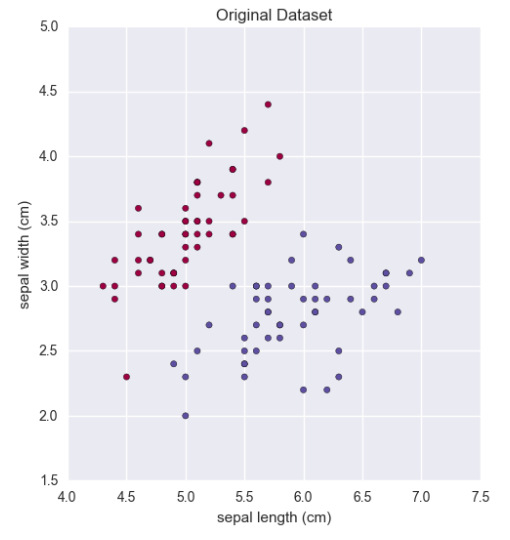
\includegraphics[width = 1.75in]{original_iris.png}\label{fig:original_iris}}
	\subfloat[][]{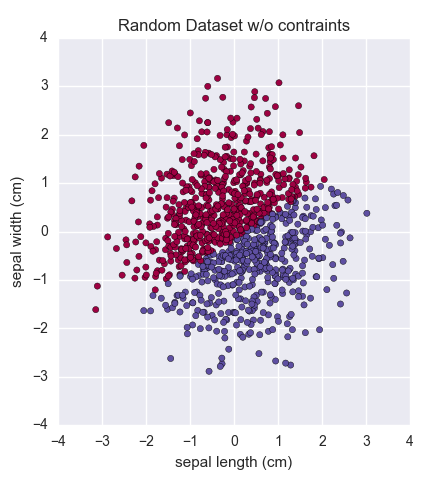
\includegraphics[width = 1.75in]{random_iris.png}\label{fig:random_iris}}
	\caption{Iris Dataset in Two Dimensions: \protect\subref{fig:original_iris} Original dataset \protect\subref{fig:random_iris} Randomly generated data}
\end{figure}

\begin{figure}[t!]
	\subfloat[][]{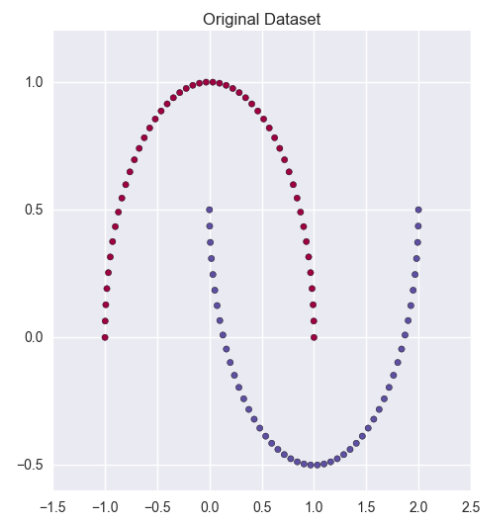
\includegraphics[width = 1.75in]{original_moons.png}\label{fig:original_moons}}
	\subfloat[][]{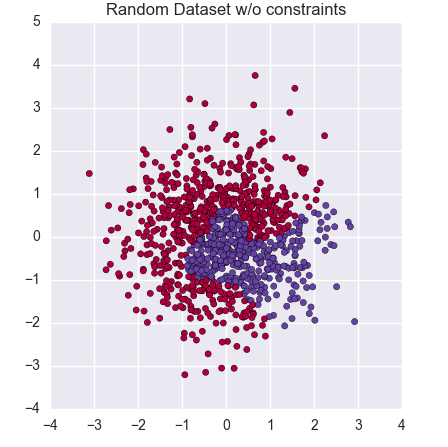
\includegraphics[width = 1.75in]{random_moons.png}\label{fig:random_moons}}
	\caption{Make Moons Dataset: \protect\subref{fig:original_moons} Original dataset \protect\subref{fig:random_moons} Randomly generated data}
\end{figure}        
% Figure ends

\subsection*{Shortcomings of the naïve approach}
Some of the shortcomings of the discussed approach are as follows
\begin{enumerate}
    \item As visualised earlier, the naïve approach does not scale well when the complexity of the data in terms of the number of features is increased. The cloned model accuracy remains lower even when the black box accuracy is quite high for the same statistical model.
    \item Since the random data generated is always derived from zero centred normal distribution, the random data won't work for models which were trained on data which does not have zero mean and unary standard deviation. This schism between the data will widen in case of nonlinear classifiers in which the hyperplane may change drastically outside the feature values.
\end{enumerate}

\section*{Generating random data under constraints}

% Procedure
Machine learning models specifically depend on the data to solve the problem. It is quite common that the data is derived from a natural phenomenon and each of the feature value thus recorded lies under a minimum and maximum value. For example, considering the Iris dataset, the sepal width and sepal length may well be under some specific range. We hypothesise that exploiting this range to generate random data can bolster the performance of our white box even in high dimensions.\\
Algorithm \ref{alg:Algorithm 2} discusses the generation of random data under constraints. The cloning procedure is rather similar and the performance of the white box is judged using the same metric.

% Algorithm 2 : Generating random data under constraints
\begin{algorithm2e}
 \KwData{blackbox , whitebox, number of features, number of samples, range of features}
 \KwResult{a cloned model}
 data = array of zeros of size [number of features, number of samples]\;
 \For{each feature in the data}{
  feature = \textbf{uniform distribution under constraints(range of feature)}\;
  label = blackbox.predict(data)\;
  whitebox.fit(data, label)\;
  // Checking the performance of the whitebox on original data\\
  print whitebox.score(original data, original labels)\;
 }
 \caption{Algorithm for cloning model using random data under constraints}
 \label{alg:Algorithm 2}
\end{algorithm2e}
% Algorithm ends

% Observations and Results for the constrained approach
The observations are summarized in table \ref{table:2}. It can be easily observed that the black box, as well as white box have almost similar accuracy for all of the datasets. If the black box tends to fail on a given dataset and the similar statistical model is used as the white box then it can be observed that the white box also performs poorly on that dataset. This provides information about the non augmenting nature of cloning. No additional strength is gained by the white box when it is being cloned. The observations favour our hypothesis that random data generated under some constraints helps the cloned model in finding the appropriate position of hyperplane and producing fairly positive results in terms of accuracy.\\

% Table for Constrained Approach
\begin{table*}
  	\centering
  	\caption{\textbf{Cloned model accuracy on original dataset when trained with random dataset under range constraints}}
	\begin{tabular}{lrlrlr}
		Dataset & No. of Features & Black Box & Black Box Accuracy & White Box & White Box Accuracy \\
	\midrule
		1. Iris & 2 & Logistic Regression & 0.99 & Logistic Regression & \textbf{0.97} \\
		2. BUPA & 7 & Logistic Regression & 0.59 & Logistic Regression & \textbf{0.57} \\
		3. Heart & 9 & Logistic Regression & 0.73 & Logistic Regression & \textbf{0.72} \\
		4. Breast Cancer & 30 & Logistic Regression & 0.95 & Logistic Regression & \textbf{0.94} \\
		5. Make Moons & 2 & Neural Network & 0.99 & Random Forest & \textbf{0.98} \\
	\bottomrule
	\end{tabular}
  	\label{table:2}
\end{table*}
% Table Ends

Figure \ref{fig:constrained_iris} and figure \ref{fig:constrained_moons} illustrates the random dataset generated by putting constraints on the data generation procedure. Unlike figure \ref{fig:random_iris} and figure \ref{fig:random_moons} the hyperplane is more clearly visible and can further provide with increased confidence to the model about the position of the hyperplane.

% Figure for Random Constrained Approach
\begin{figure}[t!]
\subfloat[][]{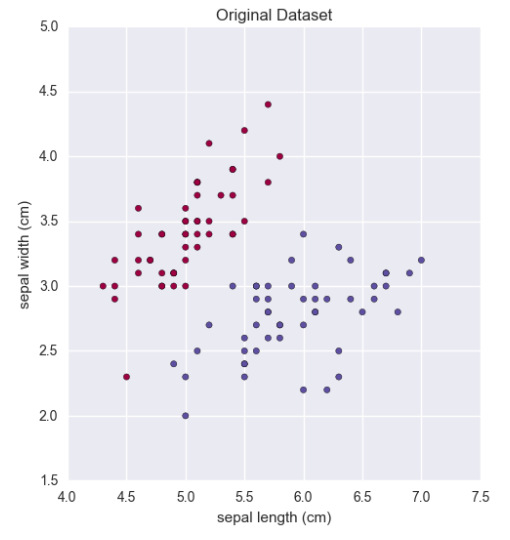
\includegraphics[width = 1.75in]{original_iris.png}\label{fig:original_iris_}}
\subfloat[][]{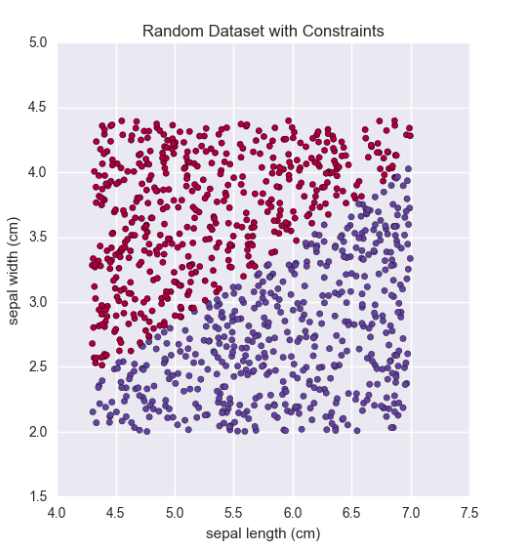
\includegraphics[width = 1.75in]{constraints_iris.png}\label{fig:constrained_iris}}
\caption{Iris Dataset in Two Dimensions: \protect\subref{fig:original_iris} Original dataset \protect\subref{fig:constrained_iris} Randomly generated data under constraints}
\end{figure}

\begin{figure}[t!]
\subfloat[][]{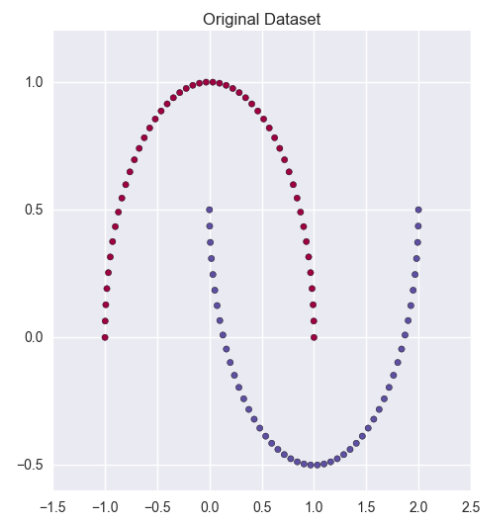
\includegraphics[width = 1.75in]{original_moons.png}\label{fig:original_moons_}}
\subfloat[][]{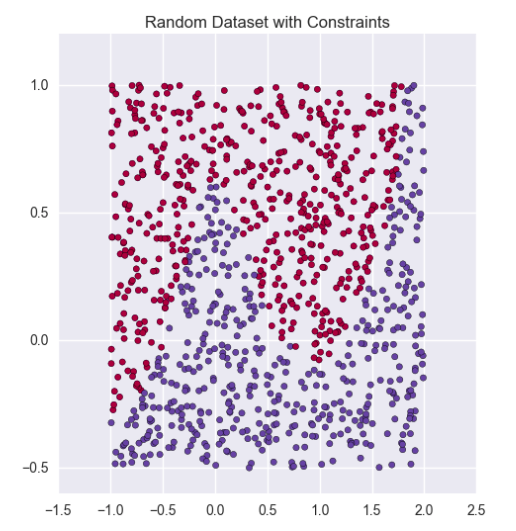
\includegraphics[width = 1.75in]{constraints_moons.png}\label{fig:constrained_moons}}
\caption{Make Moons Dataset: \protect\subref{fig:original_moons} Original dataset \protect\subref{fig:constrained_moons} Randomly generated data under constraints}
\end{figure}
% Figure ends

% Shortcomings of constrained random dataset approach
\subsection*{Shortcomings of constrained random dataset}
The only shortcoming with this approach is the \textbf{assumption that the feature values lie under some kind of constraint}. This assumption may not hold well for dataset where the data is synthetically generated or the feature can have an infinite domain.
\\
\footnotetext{Make Moons is a two dimensional non linear dataset. It was evident from its visualisation that a linear classifier would work poorly on it. So we decided to fit it with a non linear network i.e. a single hidden layer neural network with softmax outputs}

% Clonable vs Non Clonable models
\subsection*{Performance analysis of this approach on different classifiers}
Performing this experiment on a single type of linear classifier can only guarantee its effectiveness on models that perform classification using any of the parametric approaches i.e by generating the hyperplane. Apart from this, we also need to observe the accuracy of this method on non-parametric models such as Random Forest Classifier. Figure \ref{fig:modelflow} provides some new insights about this approach when it is applied on a dataset with nine features.\\
It can be observed in figure \ref{fig:modelflow} that Random Forest Classifier when used as a black box and a model to be cloned there exists a rather gap between the classification accuracy. The black box has a high accuracy whereas the white box performs poorly. This observation shows that such models (due to their non-parametric nature) can be difficult to clone and simple hyperplane approximating procedure cannot guarantee accurate cloning. Further observations need to be made to check for white box black box model interaction between Random Forests and other parametric models.

% Figure : Clonable vs Non Clonable
\begin{figure}[b!]
    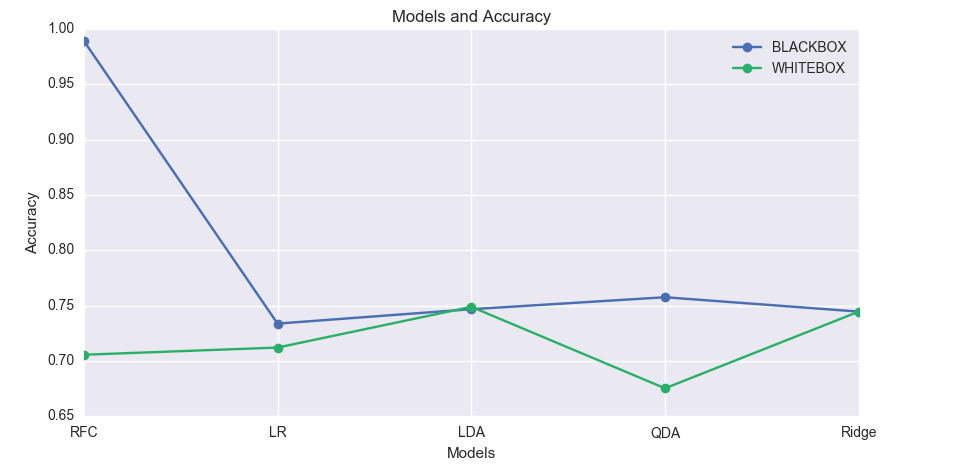
\includegraphics[width=\linewidth]{ModelFlow.png}\hfill
    \caption{Black box and White box models and their corresponding accuracy}
    \label{fig:modelflow}
\end{figure}
% Figure ends

\showmatmethods{} % Display the Materials and Methods section

\acknow{Please include your acknowledgments here, set in a single paragraph. Please do not include any acknowledgments in the Supporting Information, or anywhere else in the manuscript.}

\showacknow{} % Display the acknowledgments section

% \pnasbreak splits and balances the columns before the references.
% Uncomment \pnasbreak to view the references in the PNAS-style
% If you see unexpected formatting errors, try commenting out \pnasbreak
% as it can run into problems with floats and footnotes on the final page.
%\pnasbreak

% Bibliography
\bibliography{pnas-sample}

\end{document}